
\newcommand{\md}{\mathrm{d}}

\section{Gravitational Waves}

\subsection{Serendipitous Detections of Kilonovae}
\textit{Authors: Christian N. Setzer\footnote{christian.setzer@fysik.su.se}, Rahul Biswas, Hiranya V. Peiris}\newline
\newline
The Large Synoptic Survey Telescope (LSST) will detect millions of transients on a nightly basis \citep{LSSTScienceCollaboration2009}. This is expected to include many rare transients, such as the electromagnetic signal from the merger of two neutron stars, known as kilonovae (KNe). The coincident detection of gravitational and electromagnetic waves in 2017 \cite{TheLIGOScientificCollaboration2017, Cowperthwaite2017}, an event designated GW170817, gave us the first evidence that such kilonovae events exist, confirming long-standing predictions \citep{Li1998}. With this single event, it was possible to obtain information on cosmological parameters, yielding a measurement of the Hubble Constant: $H_0 = 70.0^{+12.0}_{-8.0} \mathrm{km\,s^{-1}\,Mpc^{-1}}$ \citep{Abbott2017}.

Given the luminosity of GW170817, and the predicted peak values of the optical/infrared after-glow from theory, we expect that it is possible to detect such events with LSST at greater distances than possible with current GW detectors \citep{Chen2017a}. What are we able to do with detections of kilonovae if we only obtain the electromagnetic counterpart? To investigate this question, it is useful to estimate how many of these events we would be able to detect. Due to the rapid evolution, short lifetime, and lower luminosity of these events we expect that the number of detectable events to be sensitive to many properties of the cadence \citep{LSSTScienceCollaboration2017}. Below we present the methods and results for our simulations of observations and detections of KNe that could be made by LSST according to different cadence prescriptions for observing the sky.

\subsubsection{Modeling}
To simulate the electromagnetic signal from KNe we separately consider two models. The only known observation of a kilonova is GW170817. To begin predicting observations, assuming the evolution of the spectral energy distribution (SED) of other kilonovae are identical to this event is a reasonable first approximation. To characterize that event we use the time-series SED, provided by the Dark Energy Survey (DES), that was used in the analysis of \citeauthor{Scolnic2017a}. This model uses multi-band photometry to calibrate a spectral time-series to observations, using photometry from \citet{Soares-Santos2017}, and
\citet{Cowperthwaite2017}.

Based on the diversity of other electromagnetic transients, it would be naive to assume that GW170817 represents the electromagnetic properties of entire range of neutron star mergers. Thus, we adopt an alternative model that is physically motivated and spans a parameter space describing a population of KNe. We have chosen a semi-analytic eigenmode expansion (SAEE) model for the SED evolution of KNe \citep{Rosswog2018}. The semi-analytic model, while one-dimensional, uses a sophisticated radiation transport treatment building on the works of \citet{Wollaeger2017} and \citet{Pinto2000}. This model uses three parameters, the gray opacity ($\kappa$), the median ejecta mass ($\mathrm{m_{ej}}$), and the median ejecta velocity ($\mathrm{v_{ej}}$) to generate the time-series SED evolution for a KN event.
\begin{table}[h!]
  \centering
  \begin{tabular}{c|c|c}
    SAEE Model Parameter & Range & Units \\
    \hline
    $\kappa$ & $\mathrm{binomial}[1, 10]$ & $\mathrm{cm^2 g^{-1}}$ \\
    \hline
    $\mathrm{m_{ej}}$ & $[0.01, 0.2]$ & $\mathrm{M_{\odot}}$ \\
    \hline
    $\mathrm{v_{ej}}$ & $[0.01, \, 0.5 (\mathrm{m_{ej}}/0.01)^{-\mathrm{log}_{20}(2)}]$ & $c$
  \end{tabular}
  \caption{The space of parameters that describe the population of KNe in the SAEE model. This range comes from the previous exploration of the parameter space in \citet{Rosswog2016a}.}
  \label{tab: ross_params}
\end{table}

The space spanned by these parameters is shown in Table \ref{tab: ross_params}, also see Fig. \ref{fig: ross_params}. For $\mathrm{v_{ej}}$, this bound was based on the condition that the total energy of the event remained under $10^{52}\, \mathrm{ergs}$. This was an upper bound adopted in the exploration of this parameter space with numerical hydrodynamics simulations, see Fig. 4 of \citet{Rosswog2016a}. The binomial distribution on the gray opacity is a standard assumption in the numerical simulation community; there is a high degree of uncertainty in this parameter for KNe \citep{Rosswog2018, Kasen2013}.

\begin{figure}[t!]
  \centering
  \includegraphics[scale=0.58]{figures/rosswog_parameter_dist}
  \caption{The parameter space of the two continuously varying parameters which characterize the population of KNe of the SAEE model. The intersection of the red lines shows where the event GW170817 falls within the parameter space for a best fit to the infrared photometric light curves,($ \mathrm{v_{ej}} = 0.15\,c\,; m_{\mathrm{ej}} = 0.06 \, M_{\odot}\,; \kappa =10 \, \mathrm{cm^2 /g}$) as determined by \citet{Rosswog2018}.}\label{fig: ross_params}
\end{figure}

To simulate observations of KNe, we begin with the number of transient events, $N_{\mathrm{total}}$, per comoving volume, $V_{\mathrm{co}}$, per event rest-frame time, $t_{\mathrm{rest}}$, which we call the comoving event rate density:

\begin{equation}\label{eqn:erd}
   \Gamma_{\mathrm{co}} =\frac{\md N_{\mathrm{total}}}{\md V_{\mathrm{co}}\, \md t_{\mathrm{rest}}}\,.
\end{equation}

This rate, $\Gamma_{\mathrm{co}}$, is assumed to be constant. We now wish to compute the redshift distribution of such events in the observer's frame and can define the distribution of events in redshift space, $n_{\mathrm{events}}$, and the cumulative number of events, $N_{\mathrm{total}}$, observed out to some redshift. These two quantities are related by

\begin{equation}\label{eqn:total_dist}
N_{\mathrm{total}}(z) = \int_0^{z} n_{\mathrm{events}}(z) \, \md z\,.
\end{equation}
Further, from Eq. \ref{eqn:erd}, we obtain
\begin{equation}
N_{\mathrm{ total}}(z) = \int_0^{T (z)} \int_0^{V_{\mathrm{co}}(z)}  \Gamma_{\mathrm{co}} \, \md V_{\mathrm{co}}(z) \,\md t_{\mathrm{rest}} \, ,
\end{equation}

where $T(z)$ is the total time elapsed in the rest frame at redshift $z$. In terms of quantities directly relatable to known properties of the observations (observation time-interval, $\Delta T_{\mathrm{obs}}$, redshift, $z$, and the sky area, $\Delta \Omega_{\mathrm{obs}}$) we find the redshift distribution

\begin{align}\label{eqn:reddist}
n_{\mathrm{events}}(z) = \, c^3  \frac{\Gamma_{\mathrm{co}}}{(1+z)H(z)} \left[\int^{z}_0 \frac{\md z'}{H(z')} \right]^2 \, \Delta T_{\mathrm{obs}} \, \Delta \Omega_{\mathrm{obs}}\,.
\end{align}

The number of observed events then follows a Poisson distribution, where $k$ are the recorded counts, and the cumulative distribution function equal to

\begin{equation}\label{eqn:invcum}
P(k;N_{\mathrm{total}}(z)) =e^{-N_{\mathrm{ total}}(z)} \sum_{i=0}^k \frac{N_{\mathrm{ total}}(z)^i}{i!}\,.
\end{equation}

Now, choosing a maximum redshift, $z_{\mathrm{max}}$, and, computing $N_{\mathrm{ total}}$, we obtain a realization of the observed events. As this is a discrete distribution, we must use an approximation of inverse of the cumulative probability distribution Eq. \ref{eqn:invcum}. This is done by randomly drawing from a uniform unit interval distribution, $u\in(0,1]$, which represents evaluations of the cumulative distribution function. Then we find the value of $k$ which gives the closest value to our draw, $u$, from the uniform distribution. This $k$ corresponds to the realization of the total number of events from the Poisson distribution, $N_{\mathrm{ total}}^{\mathrm{realization}}$. With this realization it is now possible to build a realization of the redshift distribution.

Given the cumulative redshift distribution of events, $N_{\mathrm{total}}(z)$, we scale this to the total number of events $N_{\mathrm{total}}(z_{\mathrm{max}})$. This yields a cumulative probability distribution function of transient events as a function of redshift, $F(z) = N_{\mathrm{total}}(z)/ N_{\mathrm{total}}(z_{\mathrm{max}})$. Next, we draw from a uniform unit interval distribution, $u_i\in(0,1]$, where $i$ runs from $1$ to $N_{\mathrm{ total}}^{\mathrm{realization}}$. Then, using the inverse of the cumulative distribution function, we map these draws from the uniform distribution to the redshifts which generate these values, $F^{-1}(u_i) \rightarrow z_i$. This produces a set of redshifts for all the transient events that occur within the observer frame represented by $\Delta \Omega_{\mathrm{obs}}$, $\Delta T_{\mathrm{obs}}$, and the redshift range, $z \in [0,z_{\mathrm{max}}]$.

\subsubsection{Simulations}
With the number of events and their redshift distribution calculated, we place the KNe randomly, with a uniform prior in right ascension and declination within the declination band that covers the entire LSST sky footprint for a given cadence. Additionally, the time of explosion for each event is randomly chosen with a uniform prior over the survey lifetime. This includes some buffer at the start of the survey to include events that would only overlap at the end of their evolution. Then, given a choice of KNe model, we generate a time-series SED for each event. Depending on the pairing of redshift, right ascension, and declination that it has been assigned, the SED is redshifted, dimmed, and modified with dust extinction according to the extinction map $E(B-V)$ and LSST per-bandfilter corrections from
\citet{Schlafly2011}. Each object is also assigned a peculiar velocity which Doppler-shifts the SED in the event rest frame, such that $1 + z_{\mathrm{obs}} = (1+z_{\mathrm{cosmo}})(1+z_{\mathrm{pec}})$. A summary of these parameter choices is presented in Table \ref{tab: sim_params}.

\begin{table}[h!]
\centering
\resizebox{\columnwidth}{!}{%
  \begin{tabular}{c|c|c}
  Simulation Parameter & Values & Note \\
  \hline
$z$ & $[0, 0.5]$ & $z_{\mathrm{max}}$ at Einstein Telescope Sensitivity \citep{Chen2017a}. \\
 \hline
$R_{\mathrm{KN}}$ & $1000 \mathrm{Gpc^{-3} \,yr^{-1}}$ & Rate used in \citep{Scolnic2017a}. \\
\hline
Dust Map & Per-bandfilter extinction & SFD \citep{Schlafly2011} \\
\hline
Peculiar Velocity & Gaussian($\mu = 0; \sigma = 300 \mathrm{km\, s^{-1}}$) & `Typical' values \citep{Davis2010}.
  \end{tabular}
}
 \caption{Parameters used to generate the simulated LSST kilonovae observations.}\label{tab: sim_params}
\end{table}

With this transient distribution in place, the cadence specified by an OpSim database is applied as a filtering to make observations of each event. For a given transient, all pointings that overlap with the event's spatial location and lifetime are found. Using the OpSim information such as the magnitude five-sigma limiting depth, and assuming a circular field-of-view geometry, the instrument measured flux and many other properties of the observations are computed. This set of simulated observations does not take into account realistic assumptions about our ability to discern observations of true transients. This is simulated by passing the observations through a second stage of filtering given by a set of criteria for detection.

\subsubsection{Metric}
The metric we have chosen for evaluation of a cadence is the number of KNe that are detected given the simulations of observations described above. The criteria that we use to determine detections is that of \citet{Scolnic2017a}. These criteria are the following:
\begin{itemize}
  \item Two alerts separated by $\geq 30$ minutes.
  \item Observations in at least two filters with $\mathrm{SNR} \geq 5$.
  \item Observations with $\mathrm{SNR} \geq 5$ separated by maximum 25 days.
  \item A minimum of one observation of the same location within 20 days before the first $\mathrm{SNR} \geq 5$ observation.
  \item A minimum of one observation of the same location within 20 days after the last $\mathrm{SNR} \geq 5$ observation.
\end{itemize}

In this context an alert is an observation that has an observed signal-to-noise ratio greater than five after template subtraction. This is simulated using the per-filter efficiency vs. true signal-to-noise ratio response function. As this function is unknown for LSST prior to operation, we have used the set of functions that were used for the DES Y1 analysis, given their filter-set is quite similar to LSST [R. Kessler, private communication]. The observations are filtered according to these criteria and the subset of transients which pass all conditions are labeled as detections.

These are the detection results for kilonovae using a single realization of the redshift distribution for each cadence. Each of these is itself a draw from a Poisson distribution as explained above. The uncertainty on these values is then the square root of the sample mean. For the case of one sample, this mean is the number of detections that are found per cadence, and the uncertainty on the number of detections is the square root of the numbers of detections.
\begin{figure}[h!]
  \centering
  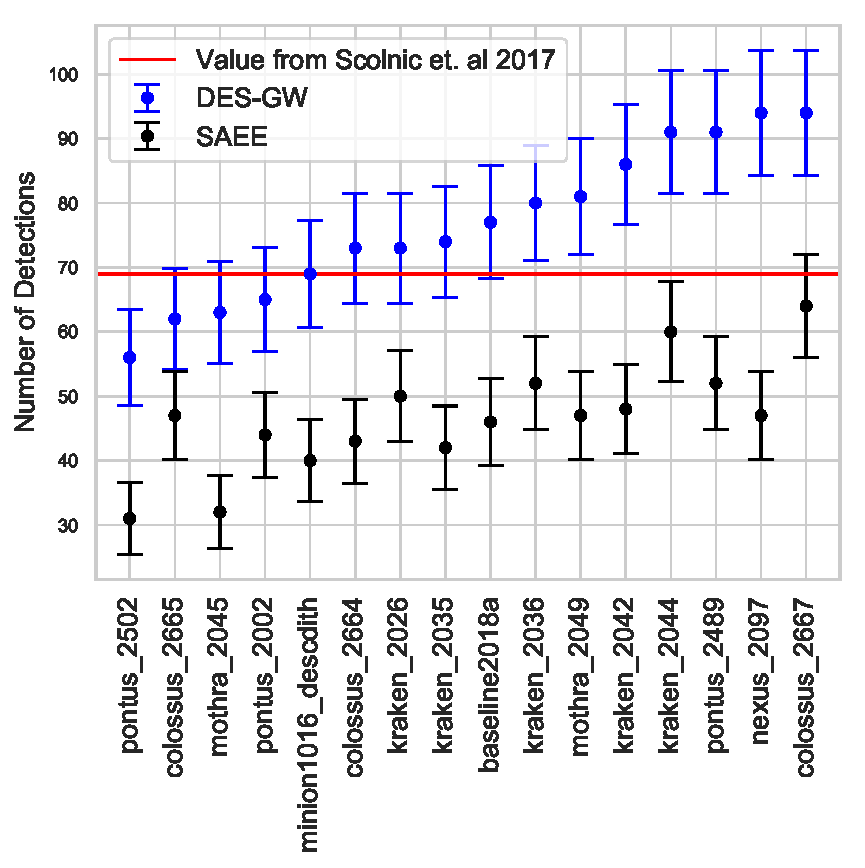
\includegraphics[scale=0.79]{figures/wfd_detection_counts_by_cadence}
  \caption{Ranking of cadence strategies for the WFD part of the survey for both KNe models, based on the number of detections found in each cadence.}
  \label{fig:cadence_ranking}
\end{figure}
\subsubsection{Results}
We rank the cadences for each KNe model based on the number of detections which pass our detections metric, see Fig. \ref{fig:cadence_ranking} and \ref{fig:cadence_ranking_ddf}. We immediately see that the DES-GW model predicts a larger number of detections than the SAEE population model. This is in part due to the early blue component, included in the DES-GW SED, being absent from the SAEE KNe model \citep{Villar2017b}. Furthermore, confirming the conclusin of \citet{Scolnic2017a}, the majority of our detections will come from the wide-fast-deep (WFD) region of the survey as opposed to the deep-drilling-fields (DDF). The typical redshift range of detected KNe, as shown in Fig. \ref{fig:typical_nz}, is between $0 \leq z \leq 0.2$, though some detections can extend out to $z \approx 0.3$. While this varies between cadences and models, this range is quite typical for all the cadences considered. The effect of changing KNe model can also be seen in Fig. \ref{fig:typical_nz}. It shows that at all redshifts the detection numbers are slightly suppressed.

\begin{figure}[h!]
  \centering
  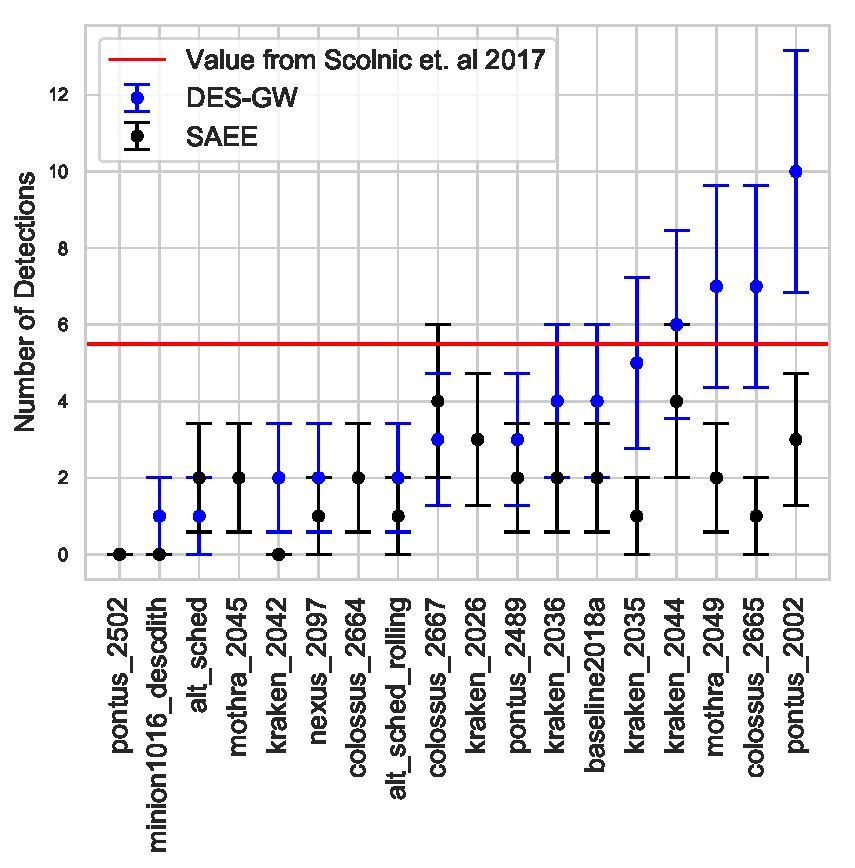
\includegraphics[scale=0.79]{figures/ddf_detection_counts_by_cadence}
  \caption{Same as the above figure, but for the DDF.}
  \label{fig:cadence_ranking_ddf}
\end{figure}

\begin{figure}[h!]
  \centering
  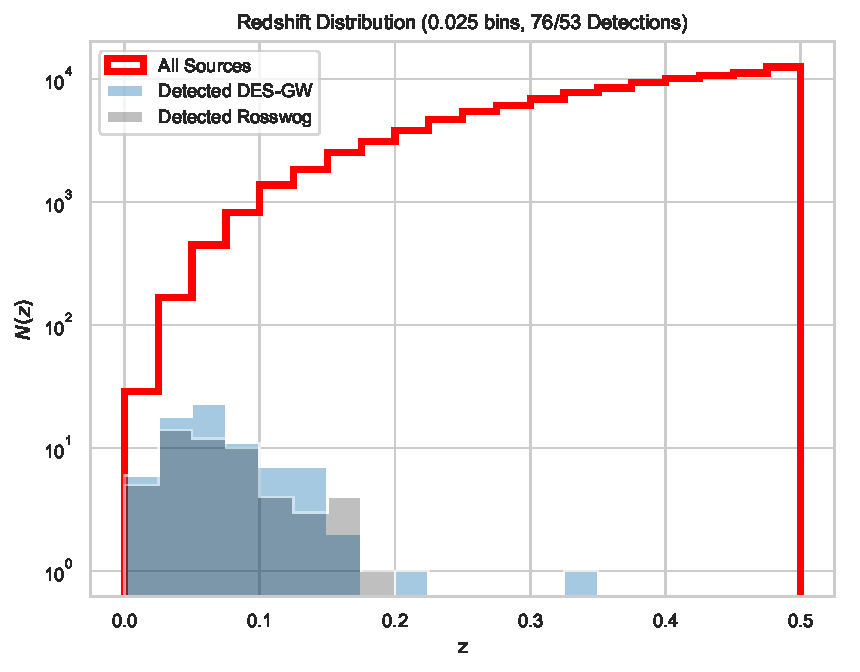
\includegraphics[scale=0.82]{figures/both_nz_base_kraken_2026}
  \caption{Example redshift distribution of detected KNe within the sample of all simulated KNe. This distribution is from the unofficial project baseline cadence \protect \textit{kraken 2026} for both the DES-GW and the SAEE KNe models. The design sensitivities of future GW detectors to detect typical binary neutron star mergers are shown by vertical lines \citep{Chen2017a, Chamberlain2017, Scolnic2017a}}
  \label{fig:typical_nz}
\end{figure}

\FloatBarrier
